% Options for packages loaded elsewhere
\PassOptionsToPackage{unicode}{hyperref}
\PassOptionsToPackage{hyphens}{url}
\PassOptionsToPackage{dvipsnames,svgnames,x11names}{xcolor}
%
\documentclass[
  letterpaper,
  DIV=11,
  numbers=noendperiod]{scrartcl}

\usepackage{amsmath,amssymb}
\usepackage{iftex}
\ifPDFTeX
  \usepackage[T1]{fontenc}
  \usepackage[utf8]{inputenc}
  \usepackage{textcomp} % provide euro and other symbols
\else % if luatex or xetex
  \usepackage{unicode-math}
  \defaultfontfeatures{Scale=MatchLowercase}
  \defaultfontfeatures[\rmfamily]{Ligatures=TeX,Scale=1}
\fi
\usepackage{lmodern}
\ifPDFTeX\else  
    % xetex/luatex font selection
\fi
% Use upquote if available, for straight quotes in verbatim environments
\IfFileExists{upquote.sty}{\usepackage{upquote}}{}
\IfFileExists{microtype.sty}{% use microtype if available
  \usepackage[]{microtype}
  \UseMicrotypeSet[protrusion]{basicmath} % disable protrusion for tt fonts
}{}
\makeatletter
\@ifundefined{KOMAClassName}{% if non-KOMA class
  \IfFileExists{parskip.sty}{%
    \usepackage{parskip}
  }{% else
    \setlength{\parindent}{0pt}
    \setlength{\parskip}{6pt plus 2pt minus 1pt}}
}{% if KOMA class
  \KOMAoptions{parskip=half}}
\makeatother
\usepackage{xcolor}
\setlength{\emergencystretch}{3em} % prevent overfull lines
\setcounter{secnumdepth}{-\maxdimen} % remove section numbering
% Make \paragraph and \subparagraph free-standing
\ifx\paragraph\undefined\else
  \let\oldparagraph\paragraph
  \renewcommand{\paragraph}[1]{\oldparagraph{#1}\mbox{}}
\fi
\ifx\subparagraph\undefined\else
  \let\oldsubparagraph\subparagraph
  \renewcommand{\subparagraph}[1]{\oldsubparagraph{#1}\mbox{}}
\fi


\providecommand{\tightlist}{%
  \setlength{\itemsep}{0pt}\setlength{\parskip}{0pt}}\usepackage{longtable,booktabs,array}
\usepackage{calc} % for calculating minipage widths
% Correct order of tables after \paragraph or \subparagraph
\usepackage{etoolbox}
\makeatletter
\patchcmd\longtable{\par}{\if@noskipsec\mbox{}\fi\par}{}{}
\makeatother
% Allow footnotes in longtable head/foot
\IfFileExists{footnotehyper.sty}{\usepackage{footnotehyper}}{\usepackage{footnote}}
\makesavenoteenv{longtable}
\usepackage{graphicx}
\makeatletter
\def\maxwidth{\ifdim\Gin@nat@width>\linewidth\linewidth\else\Gin@nat@width\fi}
\def\maxheight{\ifdim\Gin@nat@height>\textheight\textheight\else\Gin@nat@height\fi}
\makeatother
% Scale images if necessary, so that they will not overflow the page
% margins by default, and it is still possible to overwrite the defaults
% using explicit options in \includegraphics[width, height, ...]{}
\setkeys{Gin}{width=\maxwidth,height=\maxheight,keepaspectratio}
% Set default figure placement to htbp
\makeatletter
\def\fps@figure{htbp}
\makeatother

\usepackage{blkarray}
\usepackage{lineno}\linenumbers
\KOMAoption{captions}{tableheading}
\makeatletter
\@ifpackageloaded{caption}{}{\usepackage{caption}}
\AtBeginDocument{%
\ifdefined\contentsname
  \renewcommand*\contentsname{Table of contents}
\else
  \newcommand\contentsname{Table of contents}
\fi
\ifdefined\listfigurename
  \renewcommand*\listfigurename{List of Figures}
\else
  \newcommand\listfigurename{List of Figures}
\fi
\ifdefined\listtablename
  \renewcommand*\listtablename{List of Tables}
\else
  \newcommand\listtablename{List of Tables}
\fi
\ifdefined\figurename
  \renewcommand*\figurename{\textbf{Fig.}}
\else
  \newcommand\figurename{\textbf{Fig.}}
\fi
\ifdefined\tablename
  \renewcommand*\tablename{Table}
\else
  \newcommand\tablename{Table}
\fi
}
\@ifpackageloaded{float}{}{\usepackage{float}}
\floatstyle{ruled}
\@ifundefined{c@chapter}{\newfloat{codelisting}{h}{lop}}{\newfloat{codelisting}{h}{lop}[chapter]}
\floatname{codelisting}{Listing}
\newcommand*\listoflistings{\listof{codelisting}{List of Listings}}
\makeatother
\makeatletter
\makeatother
\makeatletter
\@ifpackageloaded{caption}{}{\usepackage{caption}}
\@ifpackageloaded{subcaption}{}{\usepackage{subcaption}}
\makeatother
\ifLuaTeX
  \usepackage{selnolig}  % disable illegal ligatures
\fi
\usepackage[]{natbib}
\bibliographystyle{plainnat}
\usepackage{bookmark}

\IfFileExists{xurl.sty}{\usepackage{xurl}}{} % add URL line breaks if available
\urlstyle{same} % disable monospaced font for URLs
\hypersetup{
  colorlinks=true,
  linkcolor={blue},
  filecolor={Maroon},
  citecolor={Blue},
  urlcolor={Blue},
  pdfcreator={LaTeX via pandoc}}

\author{}
\date{}

\begin{document}

\captionsetup{format=plain, labelfont=bf, labelsep=space}

\subsection{Reintroduction of resistant frogs facilitates
landscape-scale recovery in the presence of a lethal fungal
disease}\label{reintroduction-of-resistant-frogs-facilitates-landscape-scale-recovery-in-the-presence-of-a-lethal-fungal-disease}

Roland A. Knapp\textsuperscript{1,2,}*, Mark Q.
Wilber\textsuperscript{3}, Maxwell B. Joseph\textsuperscript{4,5},
Thomas C. Smith\textsuperscript{1,2} \& Robert L.
Grasso\textsuperscript{6}

\textsuperscript{1}Sierra Nevada Aquatic Research Laboratory, University
of California, Mammoth Lakes, CA, 93546

\textsuperscript{2}Earth Research Institute, University of California,
Santa Barbara, CA, 93106-3060

\textsuperscript{3}School of Natural Resources, University of Tennessee
Institute of Agriculture, Knoxville, TN, 37996

\textsuperscript{4}Earth Lab, University of Colorado, Boulder, CO, 80303

\textsuperscript{5}Current affiliation: Planet, San Francisco, CA, 94107

\textsuperscript{6}Resources Management and Science Division, Yosemite
National Park, El Portal, CA, 95318

*Corresponding author: email: roland.knapp@ucsb.edu

\subsubsection{Abstract}\label{abstract}

Vast alteration of the biosphere by humans is causing a sixth mass
extinction, driven in part by an increase in infectious diseases. The
emergence of the lethal fungal pathogen \emph{Batrachochytrium
dendrobatidis} (Bd) has devastated global amphibian biodiversity. Given
the lack of any broadly applicable methods to reverse these impacts, the
future of many amphibians appears grim. The Sierra Nevada yellow-legged
frog (\emph{Rana sierrae}) is highly susceptible to Bd infection and
most \emph{R. sierrae} populations are extirpated following disease
outbreaks. However, some populations persist and eventually recover, and
frogs in these recovering populations have increased resistance against
infection. Here, we conduct a 15-year reintroduction study and show that
frogs collected from recovering populations and reintroduced to vacant
habitats can reestablish populations despite the presence of Bd. In
addition, the likelihood of establishment is influenced by site, cohort,
and frog attributes. Results from viability modeling suggest that many
reintroduced populations have a low probability of extinction over 50
years. These results provide a rare example of how reintroduction of
resistant individuals can allow the landscape-scale recovery of
disease-impacted species, and have broad implications for amphibians and
other taxa that are threatened with extinction by novel pathogens.

\subsubsection{Introduction}\label{introduction}

Human activities are devastating global biodiversity
\citep{ceballos2015}, with important implications for ecosystem
resilience and human welfare \citep{naeem2009}. One consequence of human
alteration of the biosphere is an increase in emerging infectious
diseases \citep{jones2008, fisher2012}. Such diseases pose a severe
threat to wildlife populations \citep{daszak2000}, and have caused
dramatic declines and extinctions in a wide range of taxa, including
echinoderms, mammals, birds, and amphibians
\citep{hewson2014, samuel2015, scheele2019, cunningham2021}. Amphibians
are experiencing particularly devastating impacts of disease due to the
recent emergence and global spread of the highly virulent amphibian
chytrid fungus, \emph{Batrachochytrium dendrobatidis} (Bd)
\citep{luedtke2023, scheele2019}. By one estimate, hundreds of species
have experienced Bd-caused declines, and numerous susceptible taxa are
extinct in the wild \citep{scheele2019}. The escalating frequency of
disease emergence and the strength of impacts on wild populations
increasingly highlight the critical need for successful mitigation of
disease in species conservation.

Following pathogen arrival in a host population, resistance (ability to
limit pathogen burden) and tolerance (ability to limit the harm caused
by a particular burden) are key mechanisms by which hosts reduce disease
impacts \citep{raberg2009}. The effectiveness of these mechanisms has
direct consequences for the persistence and recovery of host populations
in the presence of disease \citep{brannelly2021}. Host immunity and
evolution both play important roles in the development of resistance and
tolerance, and are key targets for strategies aimed at mitigating
disease impacts in the wild \citep{garner2016}.

Evidence of natural recovery in the many Bd-impacted amphibian
populations is surprisingly rare (for notable exceptions, see
\citep{scheele2017, voyles2018, knapp2016}). This apparent low
resilience to disease may be due to the limited ability of many
amphibians to develop Bd resistance or tolerance via either immunity
\citep{rosenblum2012, fites2013, grogan2018a} or evolution (but see
\citep{savage2016, grogan2018b}). In turn, this would also reduce the
effectiveness of potential Bd mitigation strategies. For example, a
limited ability by amphibians to develop resistance or tolerance
suggests that reintroduction of amphibians into sites to reestablish
populations extirpated by Bd will often result not in population
recovery, but instead in the rapid reinfection and mortality of the
introduced animals and/or their progeny
\citep{hammond2021, knapp2022, stockwell2008, scheele2021}. If true, the
future of many amphibian species threatened by Bd appears bleak.

The Sierra Nevada yellow-legged frog (\emph{Rana sierrae}), is
emblematic of the global decline of amphibians caused by Bd
\citep{scheele2019}. Once the most common amphibian in the high
elevation portion of California's Sierra Nevada mountains, USA
\citep{grinnell1924}, during the past century this frog has disappeared
from more than 90\% of its historical range \citep{vredenburg2007}. Due
to the severity of its decline and the increasing probability of
extinction, \emph{R. sierrae} is now listed as ``endangered'' under the
U.S. Endangered Species Act. The decline of \emph{R. sierrae} was
initiated by the introduction of non-native trout into the extensive
fishless region of the Sierra Nevada \citep{bradford1989, knapp2000}
starting in the late 1800s. The arrival of Bd in the mid-1900s and its
subsequent spread \citep{vredenburg2019} caused additional large-scale
population extirpations \citep{vredenburg2010, rachowicz2006}. These
Bd-caused declines are fundamentally different from the fish-caused
declines because fish eradication is feasible \citep{knapp1998} and
results in the rapid recovery of frog populations
\citep{knapp2007, vredenburg2004}. In contrast, Bd appears to persist in
habitats even in the absence of amphibian hosts \citep{walker2007}, and
therefore represents a long-term alteration of invaded ecosystems that
amphibians will need to overcome to reestablish populations.

Despite the catastrophic impact of Bd on \emph{R. sierrae}, wherein most
Bd-naive populations are extirpated following Bd arrival
\citep{vredenburg2010}, some populations have persisted after epizootics
\citep{briggs2010} and are now recovering \citep{knapp2016}
(Fig.~\ref{fig-recovery-model}). During the epizootic phase, \emph{R.
sierrae} are highly susceptible to Bd infection as indicated by very
high infection intensities (``load''). In contrast, frogs in recovering
populations have reduced susceptibility to Bd infection
\citep{knapp2016}, with loads on adults consistently in the
low-to-moderate range \citep{briggs2010, knapp2011, joseph2018}. This
reduced susceptibility is evident even under controlled laboratory
conditions \citep{knapp2016}, indicative of host resistance against Bd
infection and not simply an effect of factors external to individual
frogs (e.g., environmental conditions). In addition to frogs from
recovering populations having higher resistance to Bd infection than
those from naive populations, they could also have higher tolerance, but
no data are currently available to evaluate this possibility. Therefore,
we focus on resistance throughout this paper.

The observed resistance of \emph{R. sierrae} could be the result of
several mechanisms that are not mutually exclusive, including natural
selection for more resistant genotypes \citep{savage2016, grogan2018b},
acquired immunity \citep{grogan2018a}, and/or inherent
between-population differences that pre-date Bd exposure. The possible
evolution of resistance and subsequent population recovery is consistent
with that expected under ``evolutionary rescue'', whereby rapid
evolutionary change increases the frequency of adaptive alleles and
restores positive population growth \citep{carlson2014, searle2020}.
This intriguing possibility also suggests an opportunity to expand
recovery beyond the spatial scale possible under natural recovery by
using resistant frogs from recovering populations in reintroductions to
vacant habitats \citep{joseph2018, mendelson2019}
(Fig.~\ref{fig-recovery-model}).

In the current study, we had three primary objectives. First, determine
whether the reintroduction of resistant \emph{R. sierrae}, obtained from
populations recovering from Bd-caused declines, allows the
reestablishment of populations despite ongoing disease
(Fig.~\ref{fig-recovery-model}). We accomplished this using a 15-year
large-scale reintroduction study. Second, identify important site,
cohort, and individual-level predictors of frog survival using results
from the reintroduction study. Third, estimate the probability of
persistence for the reintroduced populations over a multi-decadal
period, thereby extending our inferences of population recovery beyond
the temporal bounds of our reintroduction study
(Fig.~\ref{fig-recovery-model}). We did this using a stage-structured
matrix model (``population viability model'').

Here, we show that the majority of reintroduced populations showed
evidence of successful reproduction and recruitment despite the presence
of Bd. In addition, post-translocation frog survival is influenced by
site, cohort, and frog attributes, but not by Bd load. Finally, results
from the population viability model suggest that many reintroduced
populations have a low probability of extinction over 50 years. These
results indicate that reintroduction of resistant individuals can allow
the recovery of species driven to near-extinction by novel infectious
diseases.

\subsubsection{Results}\label{results}

\paragraph{Frog population recovery}\label{frog-population-recovery}

To determine whether \emph{R. sierrae} from recovering populations can
be used to reestablish extirpated populations, we conducted 24
reintroductions in Yosemite National Park (2006--2020). Each of the
reintroductions involved collection of adult frogs from 1 of 3
recovering, Bd-positive ``donor'' populations and translocating them to
1 of 12 nearby recipient sites (Fig.~\ref{fig-yosemap}). The 3 donor
populations are among the largest \emph{R. sierrae} populations in
Yosemite. Following translocation, we estimated adult survival and
recruitment of new adults from capture-mark-recapture (CMR) surveys and
obtained counts of tadpoles and juveniles from visual encounter surveys
(VES). Across all translocation sites, the duration of CMR surveys and
VES was 1--16 years (median = 5).

Of the 12 reintroduced populations, 9 (0.75) showed evidence of
successful reproduction in subsequent years, as indicated by the
presence of tadpoles and/or juveniles. For these 9 populations, one or
both life stages were detected in nearly all survey-years following
translocation (proportion of survey-years: median = 0.9, range =
0.29--1). These same populations were also those in which recruitment of
new adults (i.e., progeny of translocated individuals) was detected. As
with early life stages, recruits were detected in the majority of
post-translocation survey-years (proportion of survey-years: median =
0.79, range = 0.12--1). In summary, survey results indicate that
translocations resulted in the establishment of reproducing \emph{R.
sierrae} populations at most recipient sites despite the ongoing
presence of Bd.

Bd loads were fairly consistent before versus after translocation, and
loads were nearly always well below the level indicative of severe
chytridiomycosis (i.e., the disease caused by Bd) and associated frog
mortality \citep{joseph2018, vredenburg2010} (Supplementary Fig. 1).
Although it is possible that the observed relatively small changes in
load are a consequence of individuals with high Bd loads dying and
therefore being unavailable for sampling during the post-translocation
period, the fact that there was little difference in pre- versus
post-translocation Bd loads even in those populations that had very high
frog survival (70556, 74976 - see below; Supplementary Fig. 1) suggests
a true lack of substantial change in Bd load.

The ultimate measure of reintroduction success is the establishment of a
self-sustaining population. Given that it can take years or even decades
to determine the self-sustainability of a reintroduced population (for
an example in \emph{R. sierrae}, see \citep{joseph2018}), the use of
proxies is essential for providing shorter-term insights into
reintroduction success and the factors driving it. Results from our CMR
surveys allowed us to accurately estimate frog survival, including over
the entire CMR time series for each site and during only the 1-year
period immediately following translocation. These estimates were made
using site-specific models analyzed using the mrmr package
\citep{joseph2019} (\url{https://snarl1.github.io/mrmr/index.html}). We
use these estimates to describe general patterns of frog survival in all
translocated cohorts, and in an among-site meta-analysis of frog
survival to identify important predictors of 1-year frog survival (e.g.,
Bd load).

Estimates of 1-year frog survival indicate that survival was highly
variable between recipient sites, but relatively constant within
recipient sites (for the subset of sites that received multiple
translocations; Fig.~\ref{fig-translocation-survival}). These patterns
indicate an important effect of site characteristics on frog survival.
In addition, 1-year survival was higher for frogs translocated later in
the study period than earlier: 5 of the 7 populations translocated after
2013 had estimated survival \(\ge\) 0.5, compared to only 1 of 5
populations translocated prior to 2013. We suggest this resulted
primarily from our improved ability to choose recipient sites with
higher habitat quality for \emph{R. sierrae} (see \textbf{Methods - Frog
population recovery - Field methods} for details). This increased
survival has direct implications for population viability (see
\textbf{Results - Long-term population viability}).

The goal of our meta-analysis was to identify important predictors of
1-year frog survival. We were particularly interested in whether Bd load
had a negative effect on adult survival, as would be expected if frogs
were highly susceptible to Bd infection. This analysis was conducted in
a Bayesian framework and included a diversity of site, cohort, and
individual-level characteristics as predictors and 1-year frog survival
(Fig.~\ref{fig-translocation-survival}) as the response variable. The
best model of 1-year frog survival identified several important
predictors, but Bd load at the time of translocation was not among them
(Supplementary Fig. 2). Instead, important predictors included winter
severity in the year following translocation (snow\_t1), site elevation,
and donor population (Fig.~\ref{fig-cond-effects}, Supplementary Fig.
2). Males had somewhat higher survival than females, but this effect was
small (Fig.~\ref{fig-cond-effects}, Supplementary Fig. 2). The absence
of Bd load as an important predictor of frog survival is consistent with
frogs in recovering populations having sufficient resistance to suppress
Bd loads below harmful levels.

In summary, results from our frog translocation study indicate that (i)
translocations produced relatively high 1-year survival of translocated
adults, as well as reproduction and recruitment, at the majority of
recipient sites, (ii) 1-year survival of adults is influenced by site
characteristics, weather conditions, and donor population (but not Bd
load), and (iii) based on the relatively small changes in Bd load after
translocation, loads appear more strongly influenced by frog
characteristics (e.g., resistance) than site characteristics. Together,
these results indicate that frogs translocated from recovering
populations can maintain the benefits of resistance in non-natal
habitats. In addition, in 3 locations where longer CMR time series
allowed us to assess the survival of new adults recruited to the
population, naturally-recruited adults had equivalent or higher survival
probabilities than the originally translocated adults (Supplementary
Fig. 3). This suggests that frog resistance is maintained across
generations. All of the conditions described above are supportive of
population establishment and long-term population growth.

\paragraph{Long-term population
viability}\label{long-term-population-viability}

Results from the frog translocation study are suggestive of population
establishment. However, a decade or more of surveys may be necessary to
confirm that populations are in fact self-sustaining \citep{joseph2018}.
To extend our inferences of population establishment beyond those
possible from the site-specific CMR data, we developed a population
viability model. Specifically, to test whether the observed yearly adult
survival probabilities in translocated populations were sufficient for
long-term viability, we built a stage-structured matrix model that
captured known frog demography and included demographic and
environmental stochasticity. We parameterized the model using CMR data
from translocated populations and known life history values in this
system (Supplementary Table 1). Results from a sensitivity analysis are
provided in Supplementary Fig. 4.

Given observed yearly adult survival probabilities of translocated frogs
(from site-specific mrmr CMR models; provided in legend of
Fig.~\ref{fig-viability}a) and a yearly survival probability of the
year-1 juvenile class (\(\sigma_{J_1}\)) greater than 0.10, at least six
of twelve translocated populations are likely to experience a long-run
growth rate \(\lambda\) greater than 1 in the presence of Bd
(Fig.~\ref{fig-viability}a; median predicted \(\lambda\) ranges from
1.07-1.28 for these six populations). These six populations all had
observed yearly adult survival greater than 0.5. As year-1 juvenile
survival probability increased above 0.2, the deterministic long-run
growth rate of seven of twelve populations was greater than 1
(Fig.~\ref{fig-viability}a).

Even when incorporating (i) demographic stochasticity and (ii)
environmental stochasticity in year-1 juvenile survival (the transition
that we expect to be the most subject to environmental variability in
the presence of Bd), populations with high adult survival are likely to
persist over a 50 year time horizon. Our model predicted that, following
a single introduction of 40 adult individuals into a population, the six
populations with the highest adult survival probabilities
(\(\sigma_{A_R} > 0.5\)) had 50-year extinction probabilities of less
than 0.5 when the average year-1 juvenile survival was greater than 0.10
(Fig.~\ref{fig-viability}b). This indicates strong potential for
long-term persistence in the presence of Bd and environmental
variability in juvenile survival. In contrast, for the six populations
where yearly adult survival probability \(\sigma_{A_R} < 0.5\),
extinction probability over 50 years was always predicted to be
\textgreater{} 50\% regardless of the value of mean year-1 juvenile
survival between 0 and 0.25. To test the validity of our model
predictions, we demonstrated that our stochastic model could describe
the general recovery trajectory of our translocated population with the
longest survey history (Fig.~\ref{fig-viability}c; population 70550,
surveyed for 16 years).

In summary, our model demonstrates that given observed yearly adult
survival probabilities of translocated frogs, 50\% of our translocated
populations have a high probability of population growth and long-term
viability in the presence of Bd. This is likely a conservative estimate
because there is evidence that naturally-recruited adults have higher
survival probability than translocated adults (Supplementary Fig. 3),
but we considered these probabilities to be equal in all but three of
our populations where we had sufficient data to distinguish these
different probabilities.

\subsubsection{Discussion}\label{discussion}

Disease-induced population declines are decimating global biodiversity
\citep{daszak2000}, but broadly-applicable strategies to recover
affected species are generally lacking (e.g., \citep{garner2016}). Here,
we tested the possibility that populations of resistant individuals from
naturally recovering populations can be used to reestablish extirpated
populations of the endangered \emph{R. sierrae} in the presence of a
highly virulent pathogen (Bd). Our results indicate (i) the capacity of
reintroduced populations to become established and eventually recover
despite ongoing disease, (ii) that post-translocation frog survival is
influenced by site, cohort, and individual-level characteristics, and
(iii) that 50\% of the reintroduced populations are likely to persist
over a 50-year period. In light of the generally low success rate of
amphibian reintroduction efforts \citep{dodd2005}, our success in
reestablishing \emph{R. sierrae} populations via reintroduction of
resistant individuals is striking, and even more so given that \emph{R.
sierrae} was driven to near-extinction by Bd. Collectively, these
results provide a rare example of amphibian recovery in the presence of
Bd, and have important implications for the conservation and recovery of
amphibians and other taxa worldwide that are endangered by escalating
impacts from emerging infectious diseases.

Previous field studies in \emph{R. sierrae} show that frog-Bd dynamics
and frog survival in the presence of Bd are fundamentally different
between naive and recovering populations. Following the arrival and
establishment of Bd in previously-naive populations, adult frogs develop
high Bd loads that lead to mass die-offs \citep{vredenburg2010}. In
contrast, in recovering populations adult frogs typically have
low-to-moderate and relatively constant Bd loads and mass die-offs are
not observed \citep{briggs2010, knapp2011} (see also Supplementary Fig.
2). The differences in Bd load of frogs from naive and recovering
populations are also observed in controlled laboratory studies (see
Figure 4 in \citep{knapp2016}), and clearly indicate that frogs from
recovering populations exhibit resistance against Bd infection. Finally,
reintroductions of \emph{R. sierrae} collected from Bd-naive populations
and reintroduced into Bd-positive sites have consistently failed due to
the development of high Bd loads and resulting high frog mortality,
suggesting the importance of frog resistance in population
reestablishment in the presence of Bd.

In the current study, reintroduction of resistant \emph{R. sierrae} was
remarkably successful in reestablishing populations in the presence of
Bd. Of the 12 translocated populations, approximately 80\% showed
evidence of both successful reproduction and recruitment of new adults.
Year-1 survival for 12 of the 24 translocated cohorts exceeded 50\%, and
\textgreater{} 70\% of translocated cohorts had survival above this 50\%
level when the earliest translocations are excluded (i.e.,
translocations conducted when methods were still being refined; see
\textbf{Methods - Frog population recovery - Field methods} for a brief
description of these refinements). The fact that the relatively low Bd
loads and correspondingly high frog survival were both maintained when
frogs were moved from donor populations to recipient sites indicates
that these qualities of naturally-recovering populations were not solely
an effect of site characteristics, but were also strongly influenced by
intrinsic characteristics of frogs, including resistance. Although it
could be argued that the relatively invariant Bd loads before versus
after translocation are a consequence of similar pathogen pressure in
the donor and reintroduced populations, this is at odds with the fact
that in the first year after translocation frog densities are typically
1-2 orders of magnitude lower in the reintroduced versus donor
populations and pathogen pressure should follow a similar pattern. In
addition to the maintenance of Bd load and frog survival between natal
and recipient sites (Supplementary Fig. 3), the relatively high survival
of translocated frogs was maintained in their progeny, as expected if
resistance has a genetic basis.

Results from the population viability model were also encouraging. In
particular, translocated populations with \textgreater{} 50\% survival
in the first year post-translocation were predicted to have a low
probability of extinction over 50 years (probability of extinction \(<\)
0.5 when year-1 juvenile survival probability was greater than 0.10).
The viability model highlighted the important role of frog survival in
affecting long-term population viability, and allowed us to extend the
temporal scale of our study beyond the years covered by our
post-translocation surveys. These long-term forecasts are important,
given that reintroduced \emph{R. sierrae} populations may often take
decades to achieve our ultimate goal of self-sustainability
\citep{joseph2018}. Making well-supported projections about the
long-term outcome of reintroduction efforts from shorter-term
information is crucial for adaptive management of species reintroduction
programs \citep{seddon2007}, including the one we are carrying out for
\emph{R. sierrae}. Specifically, the combined results from our
reintroduction study and viability modeling suggest that survival of
frogs in the first year following translocation is an effective proxy of
longer-term survival and population viability. In addition, given the
repeatability of frog survival at a site, 1-year frog survival also
serves as an effective proxy of site quality (i.e., the ability of a
site to support high frog survival and a viable frog population over the
long term). This proxy of site quality is important in the \emph{R.
sierrae} system because accurately predicting the ability of a site to
support a viable frog population \emph{a priori} remains difficult, even
after conducting 24 translocations over 16 years.

The results of the meta-analysis indicate the influence of several
variables on adult survival, and by extension on population viability.
Although we assume that the effects of winter severity and frog sex are
direct effects of the variables themselves, the elevation and donor
population variables are likely serving as proxies for a range of
factors. For example, elevation is correlated with several attributes
that may influence frog survival, including the presence of boulder
habitat (positive correlation) that is important for frog overwintering,
abundance of frog predators including garter snakes (negative
correlation), and frog developmental rates (negative correlation). The
latter can influence the duration of frog life stages that have
differential susceptibility to chytridiomycosis (see below). The
duration of the tadpole and juvenile stages increases with elevation,
but the fact that long-run population growth rate from our viability
model is relatively insensitive to variation in these durations suggests
that developmental rates of early frog life stages have minimal effect
on the predicted long-term viability of reintroduced populations. The
mechanisms underlying the effect of donor population on the probability
of post-translocation frog survival is intriguing, and could indicate
population-specific fitness differences of frogs in the presence of Bd.
Although our study design did not allow us to completely separate the
effects of donor population and recipient site on 1-year adult survival,
we are currently doing so using a modified study design. Specifically,
we are conducting translocations in which frogs from several donor
populations are added concurrently to a single site. Survival of frogs
from each donor population is estimated using CMR methods and the
contribution of each donor population to subsequent generations is
quantified using genetic methods.

Despite the demonstrated resistance of adult \emph{R. sierrae} against
Bd infection, individual and population-level impacts of Bd are still
evident. In an earlier study of 2 of our 12 translocated populations
\citep{joseph2018}, Bd infection and load had detectable effects on the
survival of adults and may have influenced population establishment
(sites referred to as ``Alpine'' and ``Subalpine'' in \citet{joseph2018}
are identified as ``70550'' and ``70505'' in the current study).
Applying similar analyses to all 12 of our translocated populations
would likely provide a broader perspective of the ongoing effect of Bd.
In addition to these important but relatively subtle effects of Bd on
adults, the impacts on younger life stages are more apparent. \emph{R.
sierrae} immediately following metamorphosis (``metamorphs'') are highly
susceptible to Bd infection \citep{ellison2019} and as a result
experience high mortality \citep{rachowicz2006}. This high
susceptibility of metamorphs is documented in numerous species of
anurans, and may result from the poorly developed immune system
characteristic of this life stage \citep{humphries2022}. In both
naturally recovering and reintroduced \emph{R. sierrae} populations, we
suggest that the high mortality of metamorphs is an important limitation
on subsequent recruitment of new adults. Therefore, although adult
\emph{R. sierrae} appear relatively resistant, Bd infection continues to
have important limiting effects on recovering populations (see also
\citep{hollanders2022}). The ongoing high susceptibility of metamorphs
to chytridiomycosis also highlights the critical need to develop better
methods of monitoring this vulnerable life stage, the results of which
could significantly advance the conservation and recovery of Bd-impacted
amphibians.

Our successful use of translocations to reestablish \emph{R. sierrae}
populations despite ongoing Bd infection is particularly important
because natural recovery alone appears insufficient to allow
reestablishment of populations at the landscape scale. Naturally
recovering \emph{R. sierrae} populations in Yosemite are relatively rare
and are often isolated from other such populations and from suitable but
vacant habitats. This isolation is the consequence of both natural
fragmentation due to rugged geography and the ongoing presence of
introduced, predatory trout in the majority of lakes and streams
\citep{bradford1993}. Collectively, these factors often prevent
naturally recovering \emph{R. sierrae} populations from expanding via
dispersal of frogs to nearby unoccupied habitats. Translocations allowed
us to overcome these dispersal limitations and reestablish populations
in sites that would otherwise remain unoccupied for the foreseeable
future. Of particular note are the translocations that we conducted as
part of the current study into areas from which \emph{R. sierrae} were
completely extirpated, but instead of single isolated habitats these
areas contained habitats composed of interconnected fishless lakes,
ponds, marshes, and/or streams. Successful reestablishment of one
\emph{R. sierrae} population in such areas has produced a source of
frogs from which adults and juveniles are now dispersing into adjacent
habitats. This process of translocation, establishment, and subsequent
dispersal has significant potential to eventually allow the
reestablishment of robust metapopulations that may be more resilient to
current and future natural and anthropogenic impacts than more
fragmented populations (e.g., \citep{heard2015}).

The promising example provided by our study of successful
reestablishment of \emph{R. sierrae} despite ongoing Bd infection may
provide an important roadmap for ongoing and future efforts to recover
the hundreds of Bd-impacted amphibian species globally. Importantly, in
addition to the natural recovery documented for \emph{R. sierrae}
\citep{knapp2016}, other amphibian species are also showing evidence of
post-epizootic recovery in the presence of Bd
\citep{scheele2017, voyles2018} and suggest the possibility of also
using animals from these recovering populations to reestablish
extirpated populations. As with \emph{R. sierrae}, the feasibility and
long-term success of such efforts will depend on the availability of
robust donor populations containing individuals that have sufficiently
high resistance to allow frog survival and population growth in the
presence of Bd. We suggest that several components of recovery efforts
could play important roles in maximizing their success. First, an
adaptive management approach such as the one we utilized, in which the
outcomes of recovery actions are rigorously assessed and this
information is used to reduce uncertainties and inform future actions,
will often be essential \citep{canessa2019}. Second, given the apparent
rarity in amphibians of evolution of resistance against Bd infection,
developing an improved understanding of the factors facilitating or
limiting the development of frog resistance and the effectiveness of
selective breeding programs and other genetic interventions to enhance
frog resistance \citep{kosch2022} may be particularly important.
Finally, although we did not quantify the genetic structure of the donor
and translocated populations of \emph{R. sierrae} as part of the current
study, conducting genetic monitoring may be important to identify
sub-optimal genetic outcomes during establishment of translocated
populations (e.g., genetic bottlenecks) and allow timely implementation
of actions to mitigate such effects \citep{whiteley2015}.

In conclusion, we now have a proven strategy to reestablish extirpated
\emph{R. sierrae} populations. However, recovery across their large
historical range will require substantial resources over many decades.
The results of this study provide a hopeful starting point for that
endeavor and other future efforts worldwide.

\subsubsection{Methods}\label{methods}

\paragraph{Frog population recovery}\label{frog-population-recovery-1}

\subparagraph{Field methods}\label{field-methods}

The collection of data from live \emph{R. sierrae} described here
complies with all ethical regulations and was approved under the
University of California-Santa Barbara Institutional Animal Care and Use
Committe (IACUC) protocol number 478. For the 24 translocations we
conducted, we identified donor populations from which adult frogs
(\(\geq\) 40 mm snout-vent length) could be collected based on several
years of VES and skin swab collections \citep{knapp2016}, and results
from population genetic analyses \citep{poorten2017}. The populations
that we selected contained hundreds of \emph{R. sierrae} adults and
thousands of tadpoles. These relatively high abundances were the result
of recent increases following previous Bd-caused declines
\citep{knapp2016}. As is typical for recovering \emph{R. sierrae}
populations, Bd prevalence in the donor populations was high
(0.69--0.96) and Bd load (median log\textsubscript{10}(load) =
3.06--3.78 ITS copies) was two or more orders of magnitude below the
level at which frog mortality is expected
\citep{vredenburg2010, joseph2018} (log\textsubscript{10}(load)
\(\approx\) 5.78 ITS copies). Recipient sites to which frogs were
translocated were chosen based on previous \emph{R. sierrae} presence
(determined from VES and/or museum records) or characteristics that
suggested high quality habitat for this species \citep{knapp2005}. At
the beginning of this study, we had a relatively limited understanding
of the factors that affect habitat quality. In subsequent years, we
improved our site selection process by incorporating new information
about important habitat features, in particular, overwintering habitats
such as submerged boulders and overhanging banks. \emph{R. sierrae} were
absent from all recipient sites prior to the first translocation. This
determination was based on VES conducted at recipient sites over several
years (see additional details below regarding frog detectability during
VES).

We conducted 1--4 translocations per site (Fig.~\ref{fig-yosemap},
Fig.~\ref{fig-translocation-survival}) and each translocated cohort
included 18 to 99 frogs (median = 30). In preparation for each
translocation, adult frogs were collected from the donor population and
measured, weighed, swabbed, and PIT tagged. Frogs were transported to
the recipient site either on foot or via helicopter. Following release,
we visited translocated populations approximately once per month during
the summer active season to conduct diurnal CMR surveys and VES (summer
active season is generally July-August but can start as early as May and
end as late as September; range of survey dates = May-25 to Sep-29,
range of translocation dates = Jun-28 to Sep-02; median number of visits
(i.e., primary periods; see below) per summer = 2, range = 1--10). CMR
surveys allowed estimation of adult survival, recruitment of new adults,
and adult population size. VES provided estimates of tadpole and
juvenile abundance. During 2006-2012, we conducted CMR surveys on a
single day per site visit (primary period), during which we searched all
habitats repeatedly for adult frogs. Frogs were captured using handheld
nets, identified via their PIT tag (or tagged if they were untagged),
measured, weighed, swabbed, and released at the capture location. During
2013-2022, we generally used a robust design in which all habitats were
searched during several consecutive days (median number of secondary
periods per primary period = 3; range = 3--7), and frogs were processed
as described above. However, when the number of frogs detected on the
first survey day was zero or near zero, we typically conducted only a
single-day CMR survey. When using a robust design, within a primary
period, frogs that were captured during more than one secondary period
were measured, weighed, and swabbed during the first capture, and during
subsequent captures were only identified and released.

During each site visit, we conducted VES either immediately before CMR
surveys or during the first day of CMR surveys. VES was conducted by
walking the entire water body perimeter, first 100 m of each inlet and
outlet stream, and any fringing ponds and wetlands, and counting all
\emph{R. sierrae} tadpoles and juveniles. These \emph{R. sierrae} life
stages have high detectability, and counts are highly repeatable and
provide estimates of relative abundance \citep{knapp2000}.

\subparagraph{Frog counts and reproductive
success}\label{frog-counts-and-reproductive-success}

For each of the translocated populations, we used the presence of
tadpoles and/or juveniles from VES and counts of new recruits (i.e,
untagged adults) in CMR surveys to provide two measures of successful
reproduction. To calculate the proportion of years in which
tadpoles/juveniles were present at a site, we excluded surveys conducted
in the year of the initial translocation to that site. This exclusion
accounted for the fact that all translocations were conducted after the
breeding period and reproduction would therefore not occur until the
following year. Similarly, to calculate the proportion of years in which
new recruits were present at a site, we excluded surveys conducted
during the 3 years following the initial translocation. This accounted
for the multi-year tadpole and juvenile stages in \emph{R. sierrae}
(Supplementary Table 1).

\subparagraph{Estimation of frog survival and
abundance}\label{estimation-of-frog-survival-and-abundance}

For each translocation site, we estimated survival of translocated
frogs, recruitment of new frogs into the adult population, and adult
population size using a site-specific Bayesian open-population
Jolly-Seber CMR model with known additions to the population (i.e.,
translocated cohorts), as implemented by the mrmr package
\citep{joseph2019} and using R Statistical Software
\citep{rsoftware2022} (v4.4.4) (see \textbf{Supplementary Methods - Frog
population recovery - CMR model structure} for details). Briefly, the
model tracks the states of \emph{M} individuals that comprise a
superpopulation made up of real and pseudo-individuals
\citep{joseph2018}. The possible states of individuals include ``not
recruited'', ``alive'', and ``dead''. The possible observations of
individuals include ``detected'' and ``not detected''. We assume that
individuals that are in the ``not recruited'' or ``dead'' states are
never detected (i.e., there are no mistakes in the individual PIT tag
records). We also assume that new recruits were the result of
within-site reproduction and not immigration from adjacent populations.
This assumption is justified by the fact that no \emph{R. sierrae}
populations were present within several kilometers of the translocation
sites. For all models, we used mrmr defaults for priors, number of
chains (4), and warmup and post-warmup iterations (2000 for each). We
evaluated convergence of the Markov chain Monte Carlo (MCMC) algorithm
using trace plots and Gelman-Rubin statistics (Rhat).

\subparagraph{Predictors of post-translocation frog
survival}\label{predictors-of-post-translocation-frog-survival}

To identify important predictors of frog survival following
translocation, we used multilevel Bayesian models
\citep{gelman2013, gabry2019}. Included predictor variables describe
characteristics of sites, translocated cohorts, and individuals (Bd
load, sex, frog size, site elevation, winter severity in the year of
translocation, winter severity in the year following translocation,
donor population, day of year on which a translocation was conducted,
and translocation order). We used 1-year post-translocation survival
estimates from CMR models as the response. Estimated survival was
rounded to integer values to produce a binary outcome, and modeled with
a Bernoulli distribution. Group-level (random) effects included
site\_id, translocation\_id, or translocation\_id nested within
site\_id. We performed all analyses with the rstanarm package
\citep{rstanarm2022} and R Statistical Software \citep{rsoftware2022}
(v4.4.4). For all models, we used default, weakly informative priors,
four chains, and 5000 iterations each for warmup and post-warmup. We
checked MCMC convergence using trace plots and Rhat, and evaluated model
fit using leave-one-out cross-validation \citep{vehtari2016}, as
implemented by the loo package \citep{vehtari2022}. (See
\textbf{Supplementary Methods - Frog population recovery - Among-site
survival modeling} for details.)

\subparagraph{Changes in Bd load following
translocation}\label{changes-in-bd-load-following-translocation}

We analyzed skin swabs using standard Bd DNA extraction and qPCR methods
\citep{boyle2004} (see \textbf{Supplementary Information - Frog
population recovery - Laboratory methods} for details). To assess the
magnitude of changes in Bd load on frogs following translocation, we
compared Bd loads measured before versus after translocation.
Before-translocation loads were quantified using skin swabs collected
from all to-be-translocated frogs at the donor site on the day before or
the day of the translocation. After-translocation Bd loads were based on
all swabs collected from translocated frogs at the recipient site in the
year of and the year following translocation. Individual frogs and their
associated Bd loads were included in the dataset only if frogs were
captured at the recipient site at least once during the 1-year period
following translocation.

\paragraph{Population viability
modeling}\label{population-viability-modeling}

\subparagraph{Model description}\label{model-description}

To determine the implications of observed 1-year adult survival on the
long-term viability of populations established via translocation, we
developed a population model for \emph{R. sierrae}. Our central question
was: How does the magnitude and variation in observed adult survival
probability across translocated populations affect the long-term
persistence probability of populations? We developed a model that
tracked seven state variables of a frog population: abundance of
translocated adults (\(A_T\)), abundance of adults naturally recruited
into the population (\(A_R\)), abundance of first-year tadpoles
(\(L_1\)), abundance of second-year tadpoles (\(L_2\)), abundance of
third-year tadpoles (\(L_3\)), abundance of first-year juveniles
(\(J_1\)), and abundance of second-year juveniles (\(J_2\)). We divided
adults into two classes \(A_T\) and \(A_R\) because there is evidence
that the survival probability of translocated adults and naturally
recruited adults differs (Supplementary Fig. 3). The modeled population
included both male and female frogs.

We modeled the dynamics of these seven state variables using a
discrete-time, stage-structured model where a time step is one year. The
dynamics are given by

\begin{equation}\phantomsection\label{eq-matrix}{
\begin{aligned}
\begin{bmatrix}
L_1 \\
L_2 \\
L_3 \\
J_1 \\
J_2 \\
A_R \\ 
A_T
\end{bmatrix}(t + 1) = 
\begin{bmatrix}
  0 & 0 & 0 & 0 & 0 & \sigma_{A_R} p_F \rho F & \sigma_{A_T} p_F \rho F \\
  \sigma_{L1} p_{L1} & 0 & 0 & 0 & 0 & 0 & 0 \\
  0 & \sigma_{L2} p_{L2} & 0 & 0 & 0 & 0 & 0\\
  \sigma_{L1} (1 - p_{L1}) & \sigma_{L2} (1 - p_{L2}) & \sigma_{L3} & 0 & 0 & 0 & 0 \\
  0 & 0 & 0 & \sigma_{J1} p_{J1} & 0 & 0 & 0 \\
  0 & 0 & 0 & \sigma_{J1} (1 - p_{J1}) & \sigma_{J2}  & \sigma_{A_R} & 0 \\
  0 & 0 & 0 & 0 & 0 & 0 & \sigma_{A_T} 
\end{bmatrix} \begin{bmatrix}
L_1 \\
L_2 \\
L_3 \\
J_1 \\
J_2 \\
A_R \\
A_T \\
\end{bmatrix}(t) \\
\hspace{0.0001cm}
\end{aligned}
}\end{equation}

The parameters in this model are yearly survival probability
\(\sigma_{\cdot}\) (the subscript ``\(\cdot\)'' indicates a particular
state variable), probability that a female frog reproduces in a given
year \(p_F\), the percentage of adults that are female \(\rho\), number
of eggs produced by a female frog in a year that successfully hatch
\(F\), probability of a first-year tadpole remaining as a tadpole
\(p_{L1}\), probability of a second-year tadpole remaining as a tadpole
\(p_{L2}\), and probability of a first-year juvenile remaining as a
juvenile \(p_{J1}\). First-year juvenile survival \(\sigma_{J1}\) is the
parameter that we think is most influenced by environmental
stochasticity.

In this model we ignore density-dependent recruitment because we were
interested in the growth of the population from an initial
reintroduction and whether this growth was sufficient to prevent
extinction over 50 years following the introduction. We also did not
directly consider the dynamics of Bd in this model. We made this
decision because (i) translocated populations are infected with Bd at
high prevalence \citep{joseph2018}, and (ii) host density does not seem
to play a significant role in multi-year Bd infection dynamics in this
system \citep{wilber2022}. Thus, ignoring Bd infection dynamics and
instead assuming all host vital rates are in the presence of high Bd
prevalence significantly simplifies the model without much loss of
realism. Additional details are provided in \textbf{Supplementary
Methods - Population viability modeling - Incorporating yearly
variability in survival rates} and \textbf{Estimating model parameters}.

\subparagraph{Model analysis}\label{model-analysis}

After parameterizing our model with CMR-estimated adult frog survival
probabilities and other known vital rates (Supplementary Table 1), we
performed four analyses. First, we compute the long-run growth rate
\(\lambda\) for each of our 12 translocated populations to determine if
the populations were deterministically predicted to grow or decline in
the long-run. Second, we compute the elasticity and sensitivity of
\(\lambda\) to nine model parameters to quantify how much changes in
these parameters affected the long-run growth rate (Supplementary Fig.
4). This also helped us determine where in the model environmental
variation in juvenile survival would have the largest effects on
population dynamics. Third, we included demographic stochasticity and
environmental stochasticity in \(\sigma_{J_1}\) in our model and
simulated the 50-year viability (i.e., 1 - extinction probability) of
populations given an introduction of 40 adult individuals into an
unoccupied habitat. Finally, we fit our model to our longest
translocation trajectory to confirm that our model could reasonably
reproduce the observed recovery trajectories of \emph{R. sierrae}
following reintroductions. Additional details are provided in
\textbf{Supplementary Methods - Population viability modeling - Model
analysis and simulation}.

\subsubsection{Data availability}\label{data-availability}

The data used in this study are available at
\url{https://doi.org/10.5281/zenodo.13851590} \citep{knapp2024a}. This
includes the estimated survival of each reintroduced frog cohort, data
used to identify predictors of 1-year frog survival, data used to
estimate growth rates and extinction probabilities of reintroduced
populations, Bd loads on frogs before and after translocation, and
survival probabilities of translocated versus naturally recruited
adults. For the relevant figures, source data are provided in a Source
Data file. The CMR datasets from each reintroduction site that we used
to calculate post-translocation frog survival are available at
\url{https://doi.org/10.5281/zenodo.13851652} \citep{knapp2024b}.

\subsubsection{Code availability}\label{code-availability}

R code to replicate our analyses is available at
\url{https://doi.org/10.5281/zenodo.13851590} \citep{knapp2024a}. R code
to analyze the CMR datasets is available at
\url{https://doi.org/10.5281/zenodo.13851652} \citep{knapp2024b}.

\subsubsection{References}\label{references}

\renewcommand{\bibsection}{}
\bibliography{translocation.bib}

\newpage

\subsubsection{Acknowledgements}\label{acknowledgements}

We thank the following for important contributions to this study: E.
Hegeman and A. Lindauer (project and data management, field and
laboratory work); A. Barbella and K. Rose (laboratory work); numerous
summer technicians (field work); staff at Sequoia-Kings Canyon and
Yosemite National Parks, Inyo and Sierra National Forests, California
Department of Fish and Wildlife, U.S. Fish and Wildlife Service, Sierra
Nevada Aquatic Research Laboratory (DOI: 10.21973/N3966F), and
University of California-Santa Barbara Institutional Animal Care and Use
Committee (research permits, logistical support, and/or field
assistance). This project was supported by grants from the National Park
Service (to R.A.K.), Yosemite Conservancy (to R.A.K.), and National
Science Foundation (EF-0723563, to C. Briggs; DEB-1557190, to C. Briggs;
DEB-2133401, to M.Q.W; and DBI-2120084, to C. Richards-Zawacki).

\subsubsection{Author contributions}\label{author-contributions}

R.A.K., M.Q.W., M.B.J., T.C.S., and R.L.G designed the research. R.A.K.,
M.B.J., T.C.S., and R.L.G. contributed to data collection; M.B.J.
contributed new analytic tools; R.A.K. and M.Q.W. conducted the
analyses. R.A.K. and M.Q.W. wrote the manuscript with input from M.B.J.,
T.C.S., and R.L.G.

\subsubsection{\texorpdfstring{\textbf{Competing
interests}}{Competing interests}}\label{competing-interests}

The authors declare no competing interests.

\subsubsection{Additional information}\label{additional-information}

\textbf{Supplemental information} is available for this paper at

\textbf{Correspondence} and requests for materials should be addressed
to R.A.K.

\newpage

\subsubsection{Figures and Legends}\label{figures-and-legends}

\begin{figure}

\centering{

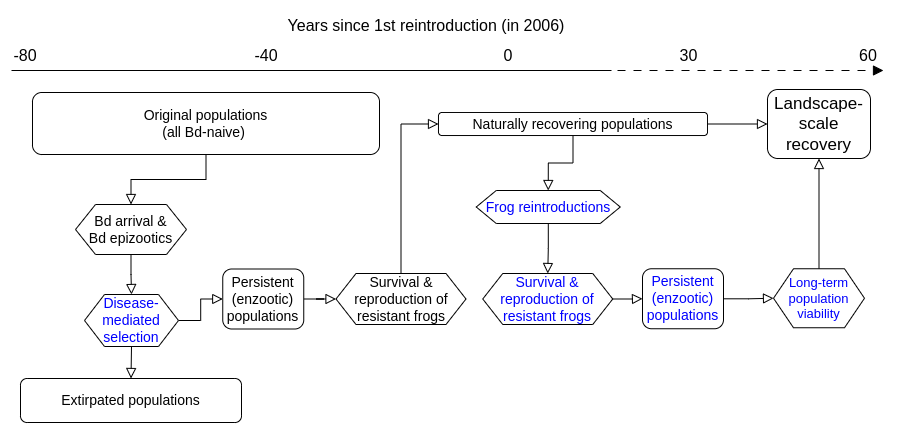
\includegraphics[width=0.95\textwidth,height=\textheight]{figures/conceptual_model.png}

}

\caption{\label{fig-recovery-model}\textbf{Conceptual model of Bd-caused
decline and recovery in \emph{R. sierrae}.} For the recovery portion,
the model depicts both natural recovery and facilitated recovery via
reintroductions, as well as the linkages between these two pathways.
Rectangles and hexagons represent outcomes and processes, respectively.
Blue text indicates components that are included in the current study.
The general temporal scale of the depicted scenario is provided by the
timeline, with the dashed portion indicating a projection into the
future.}

\end{figure}%

\newpage

\begin{figure}

\centering{

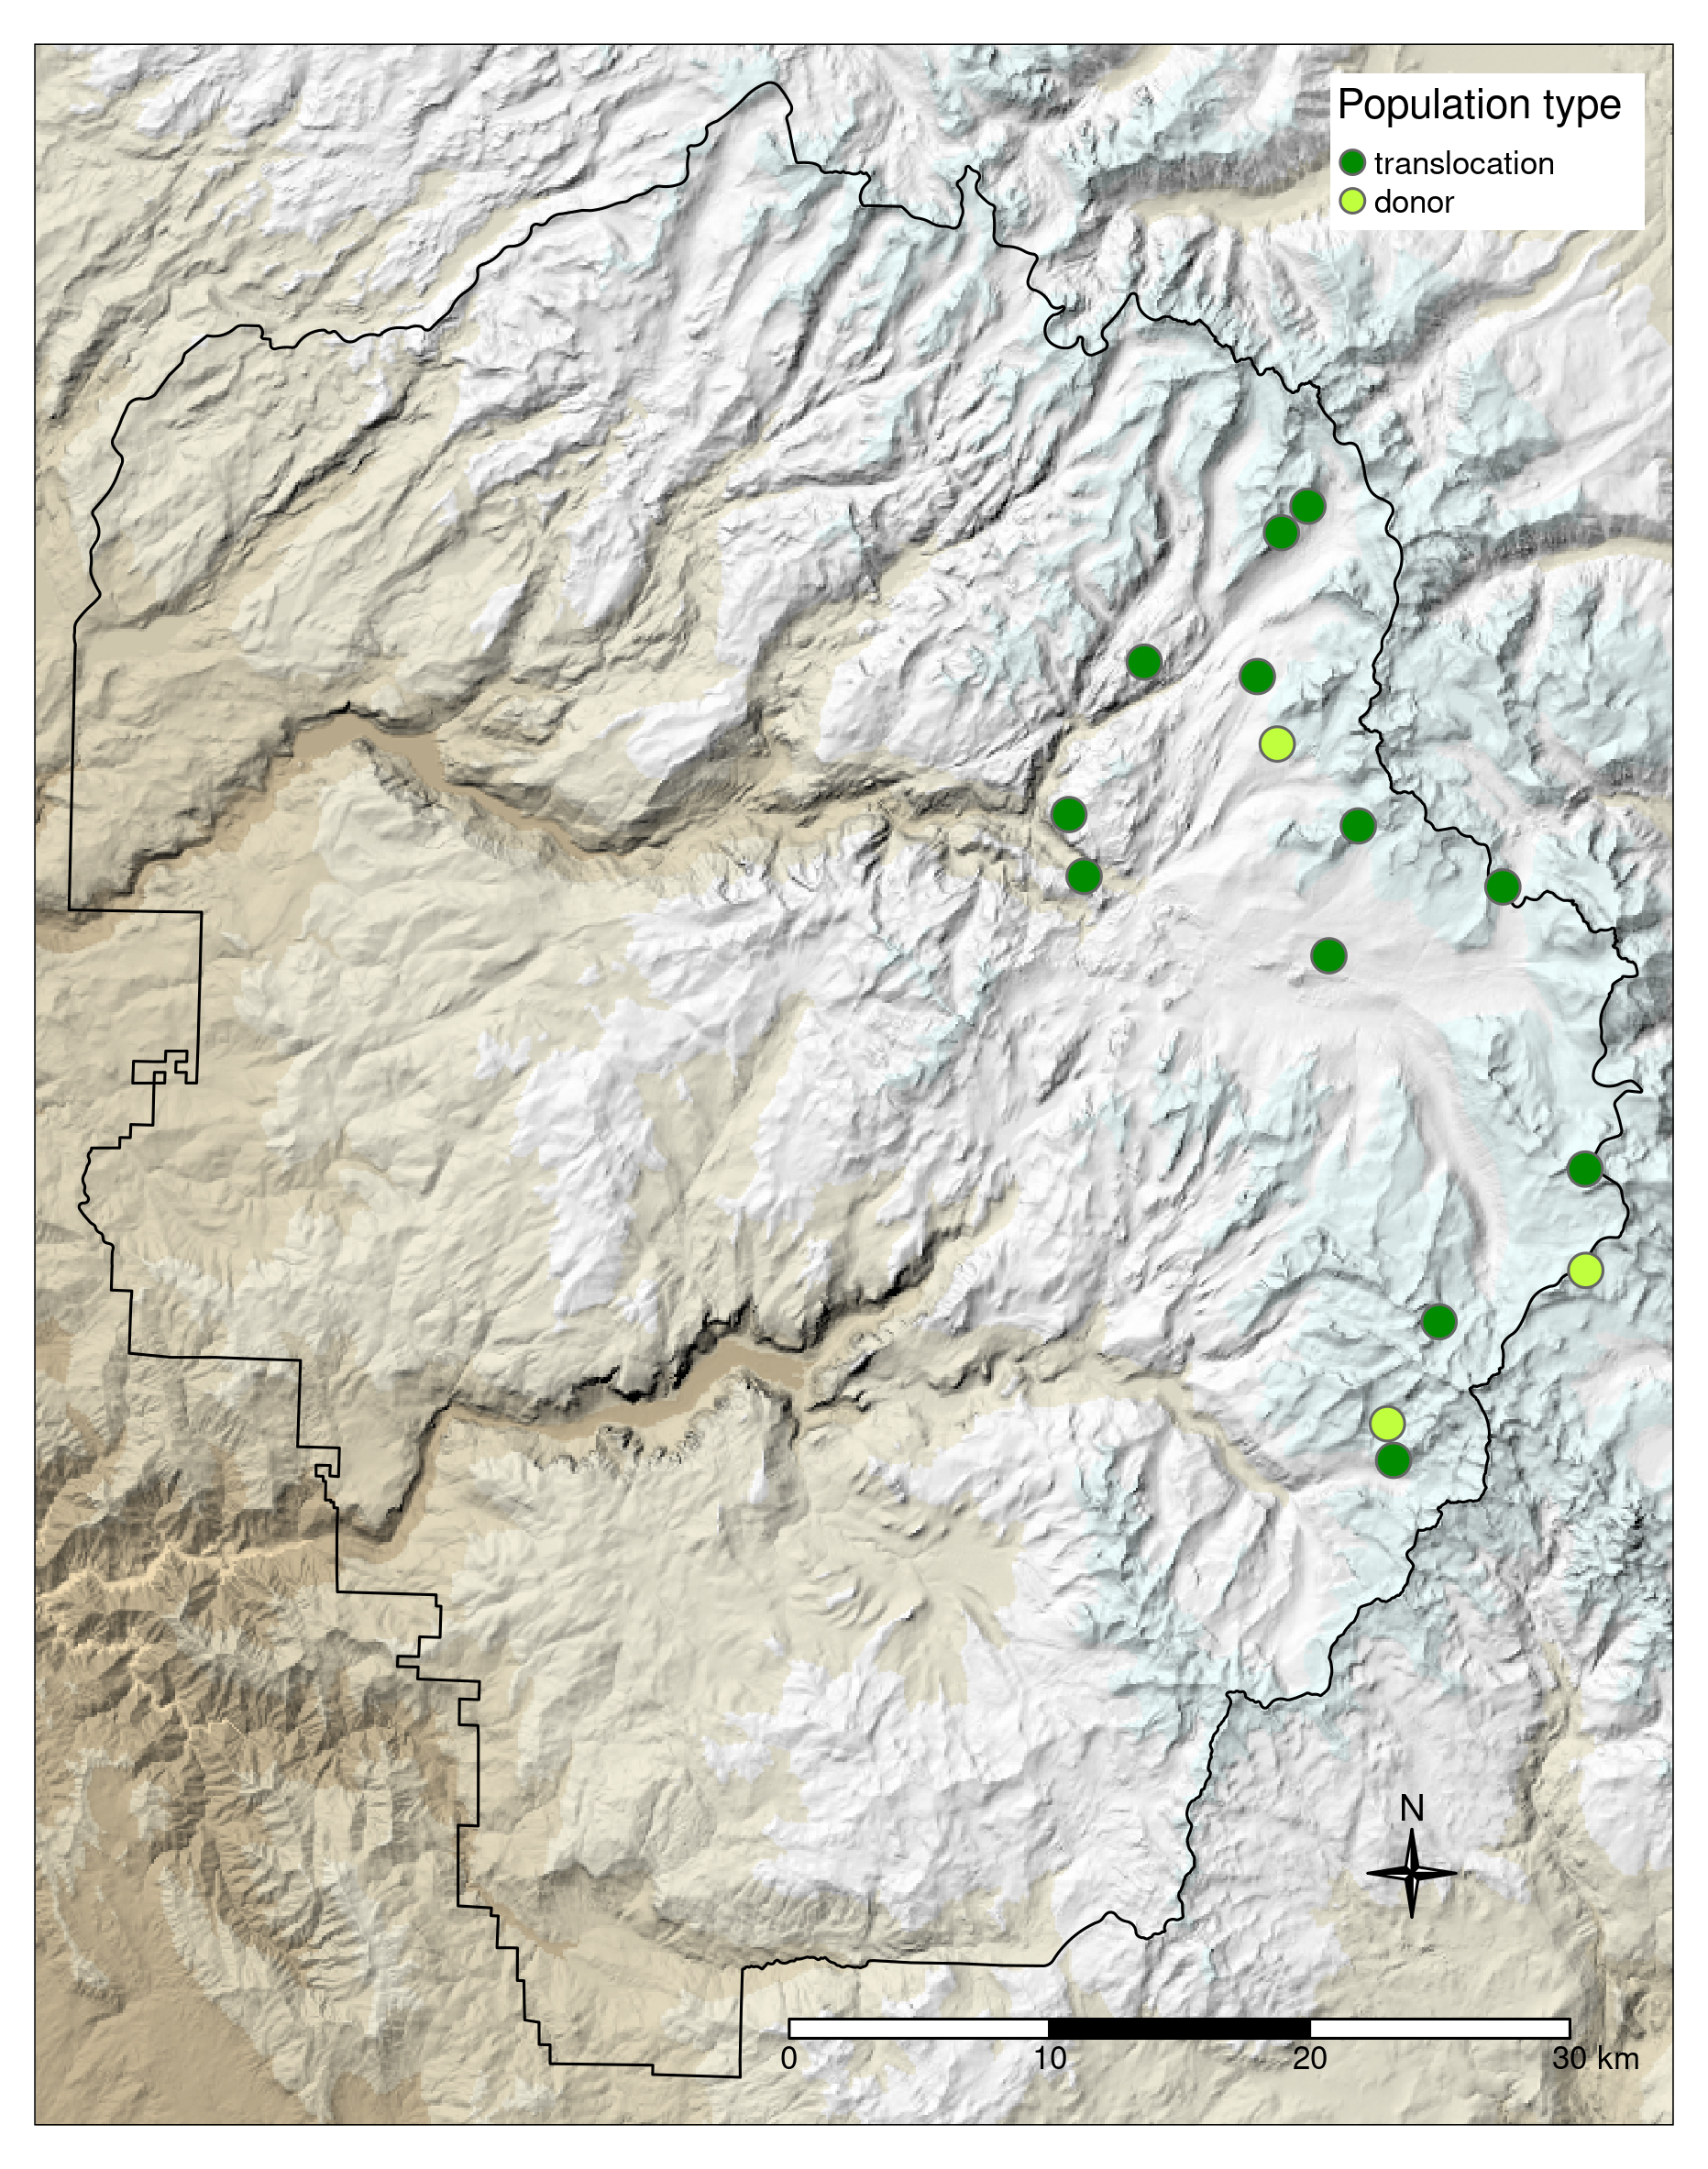
\includegraphics[width=0.6\textwidth,height=\textheight]{figures/map_translocation_points.png}

}

\caption{\label{fig-yosemap}\textbf{Locations of translocated and donor
\emph{R. sierrae} populations.} All populations are in Yosemite National
Park (park boundary indicated by black polygon). Symbol shapes indicate
the donor population used for each translocation site, and 5-digit
numbers identify each donor and translocation site. To obscure the exact
locations of populations, random noise was added to all point
coordinates. Inset map shows the location of Yosemite within California.
In both maps, topography is shown with a grayscale hillshade layer, and
elevation is indicated by colors layered over the hillshade. In the
absence of hillshading, dark green colors indicate the lowest elevations
and white indicates the highest elevation.}

\end{figure}%

\newpage

\begin{figure}

\centering{

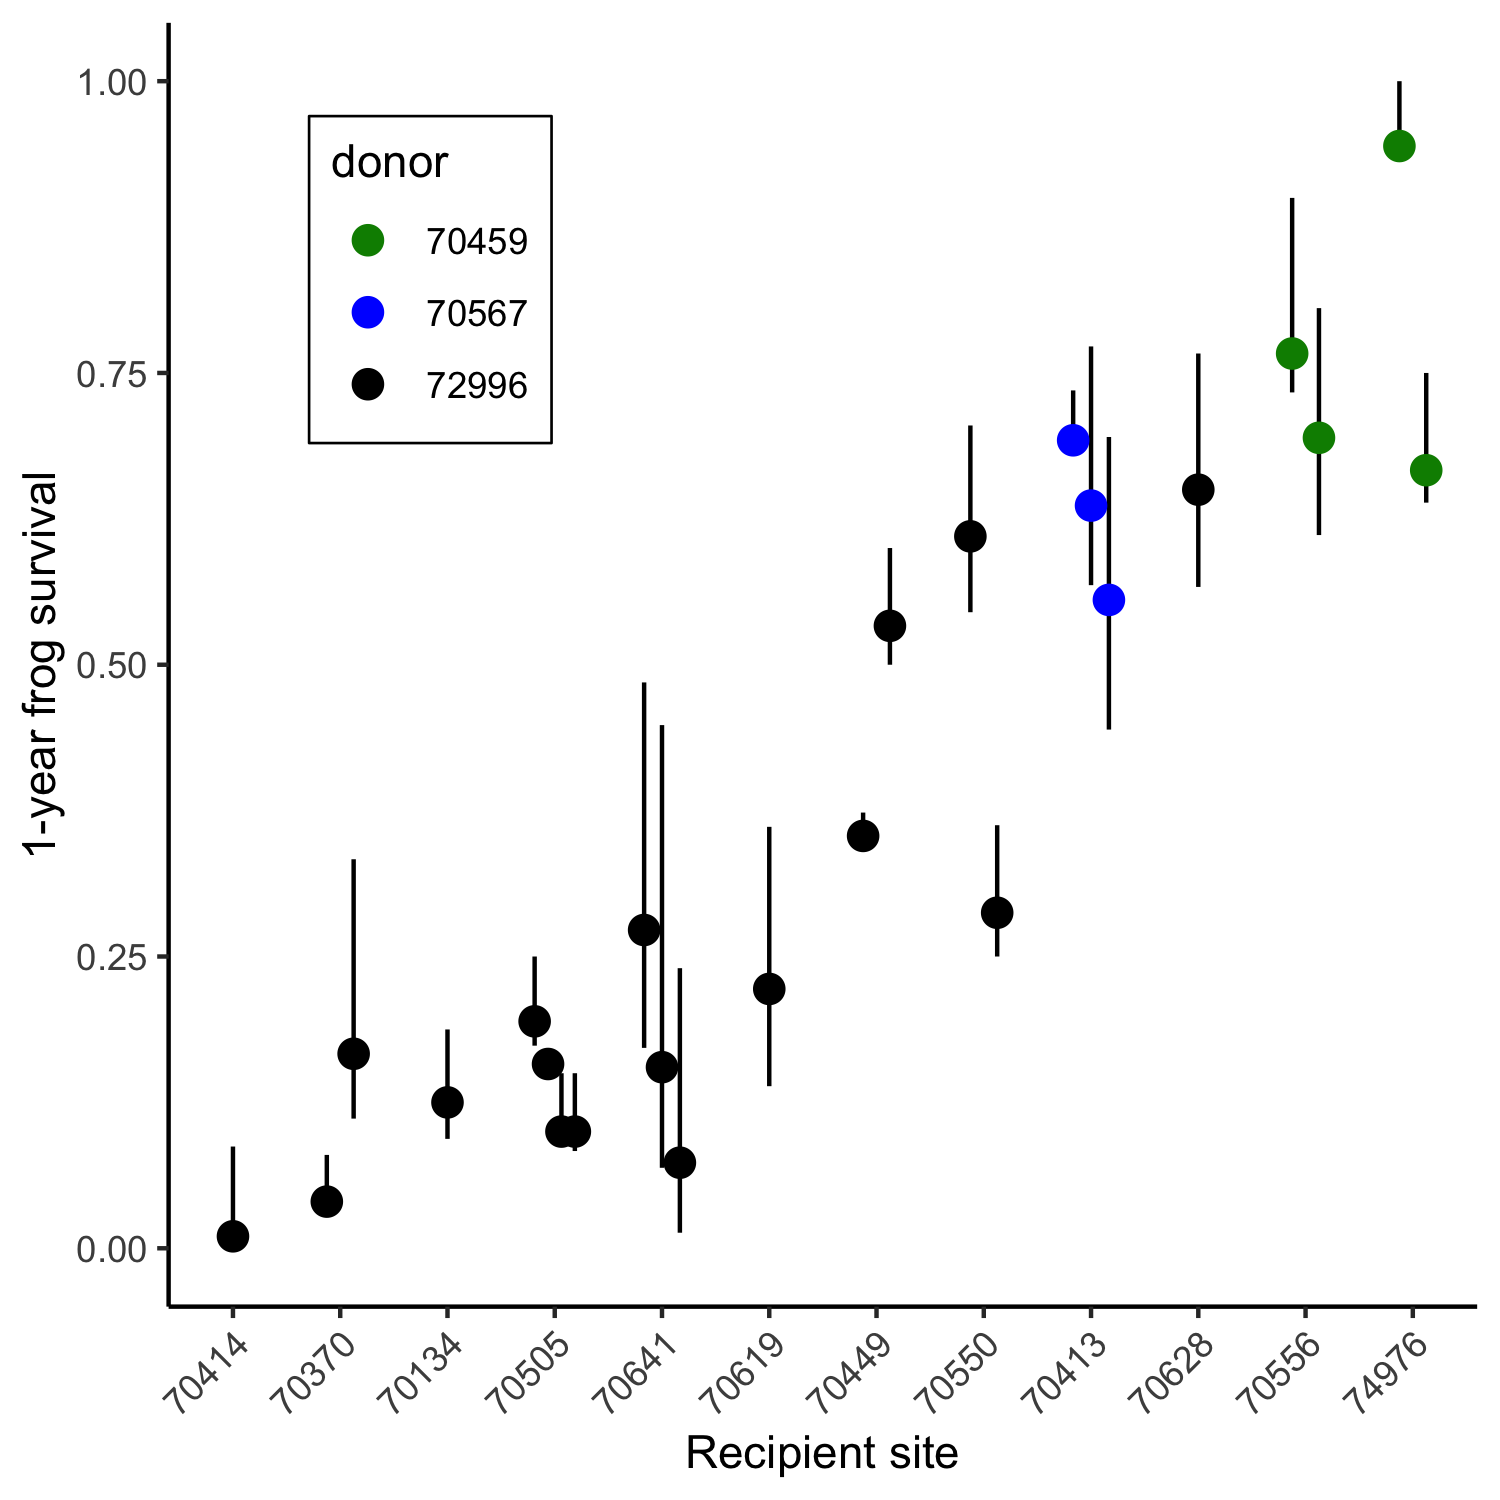
\includegraphics[width=0.6\textwidth,height=\textheight]{figures/translocation_survival_bysiteid.png}

}

\caption{\label{fig-translocation-survival}\textbf{1-year survival for
each cohort of translocated frogs}. Median cohort-level survival was
estimated for each of the 12 recipient sites using mrmr CMR models.
Error bars show the 95\% uncertainty intervals. Sites are arranged along
the x-axis using the average of the median 1-year survival per
translocation at each site. Dot colors indicate the donor population
from which frogs in each translocated cohort were collected. When
multiple translocations were conducted to a site, points and error bars
are slightly offset to avoid overlap.}

\end{figure}%

\newpage

\begin{figure}

\centering{

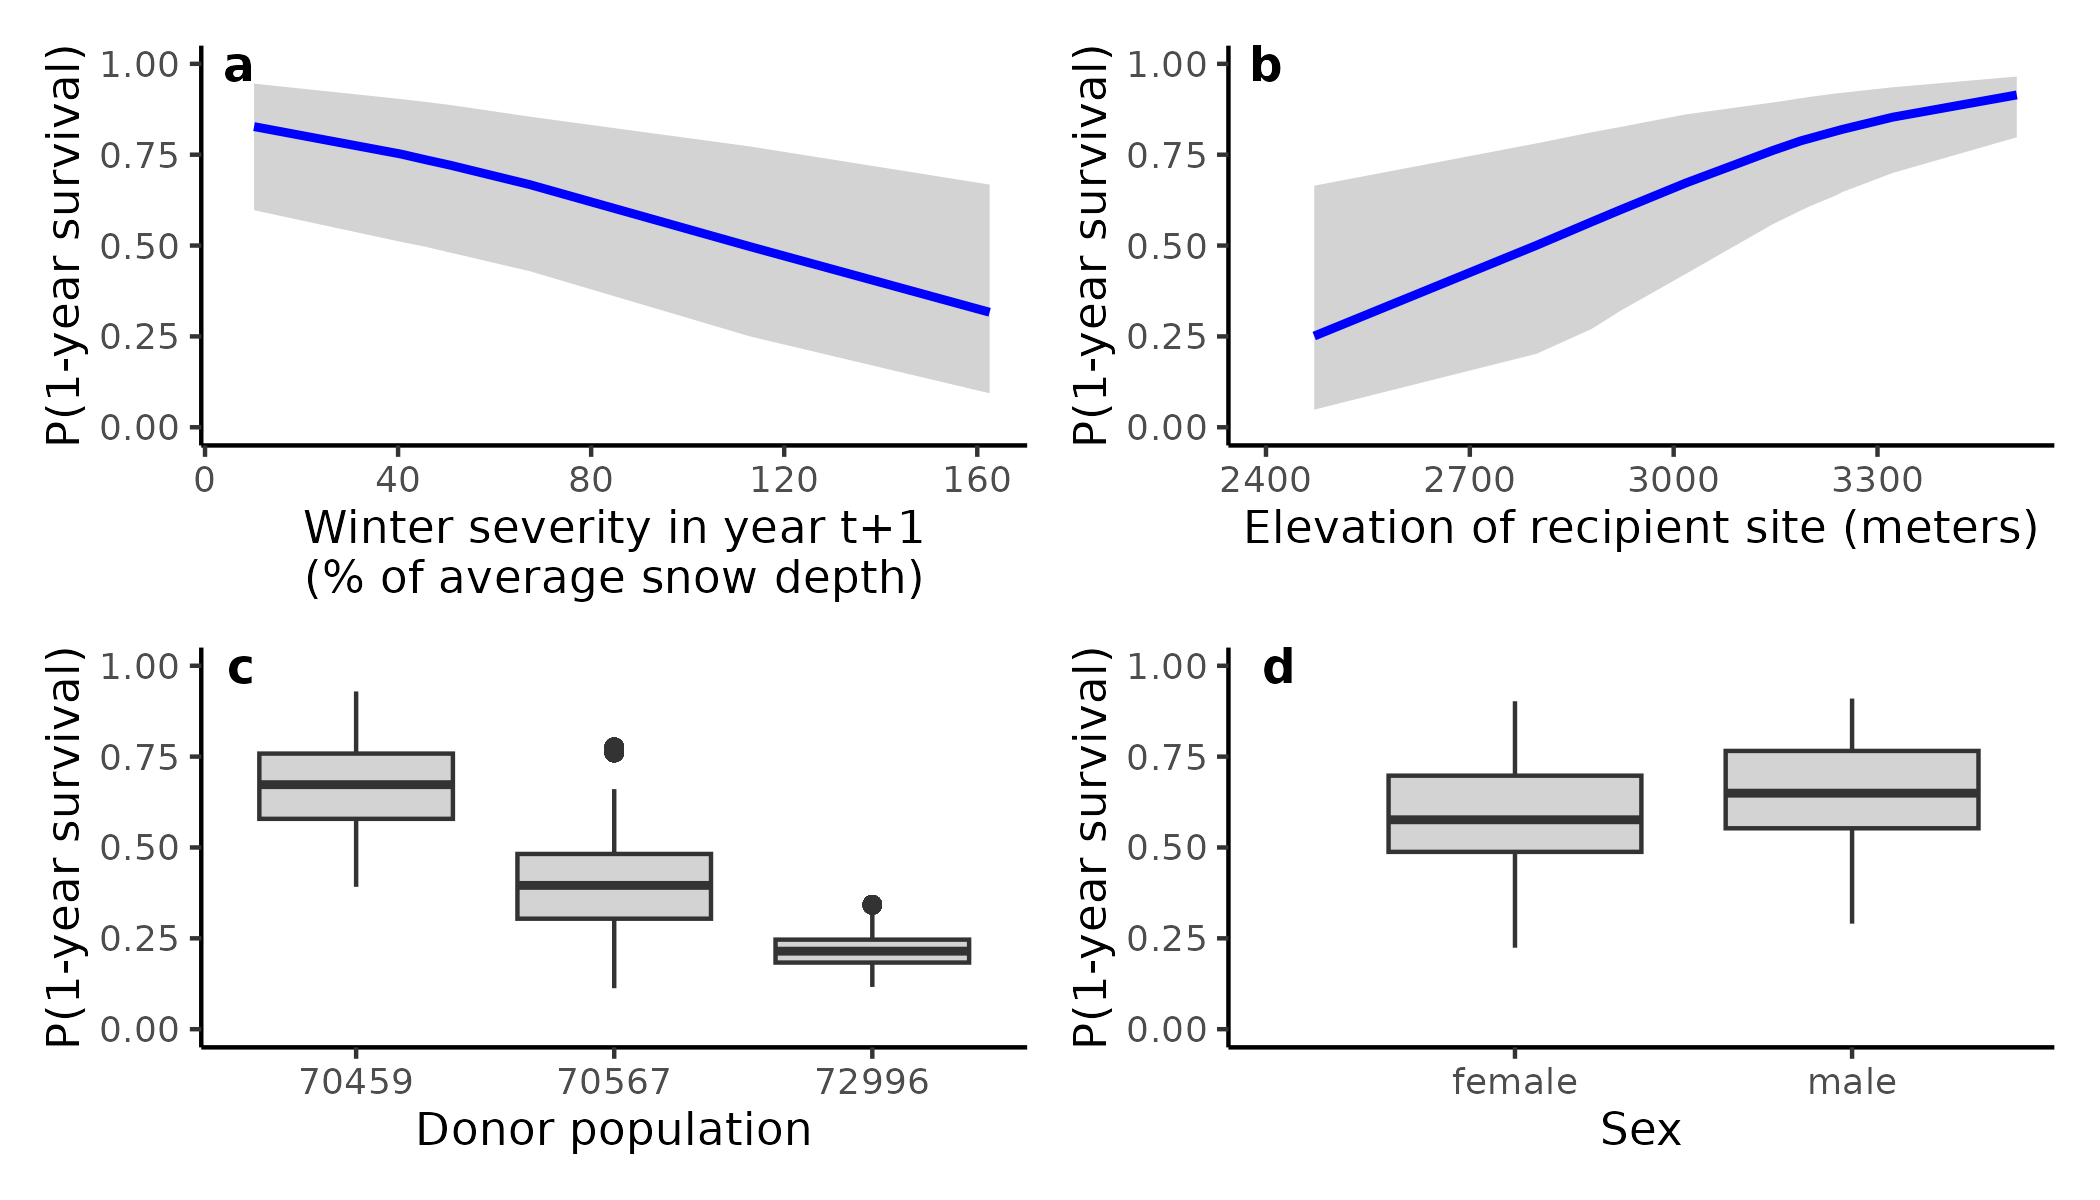
\includegraphics[width=0.8\textwidth,height=\textheight]{figures/cond_effects_plot.png}

}

\caption{\label{fig-cond-effects}\textbf{Conditional effects of
predictors of 1-year frog survival}. Results are from the among-site
meta-analysis and 1-year frog survival is expressed as a probability.
\textbf{a} winter severity in the year following translocation,
\textbf{b} elevation of recipient site, \textbf{c} donor population, and
\textbf{d} sex. In (a) and (b), blue lines are medians and gray ribbons
are 95\% uncertainty intervals for the posterior distributions of the
predicted effects. In (c) and (d), box plots show medians (horizontal
line), first and third quartiles (hinges), largest and smallest values
within 1.5x interquartile range (whiskers), and values outside the 1.5x
interquartile range (dots) for the posterior distributions of the
predicted effects.}

\end{figure}%

\newpage

\begin{figure}

\centering{

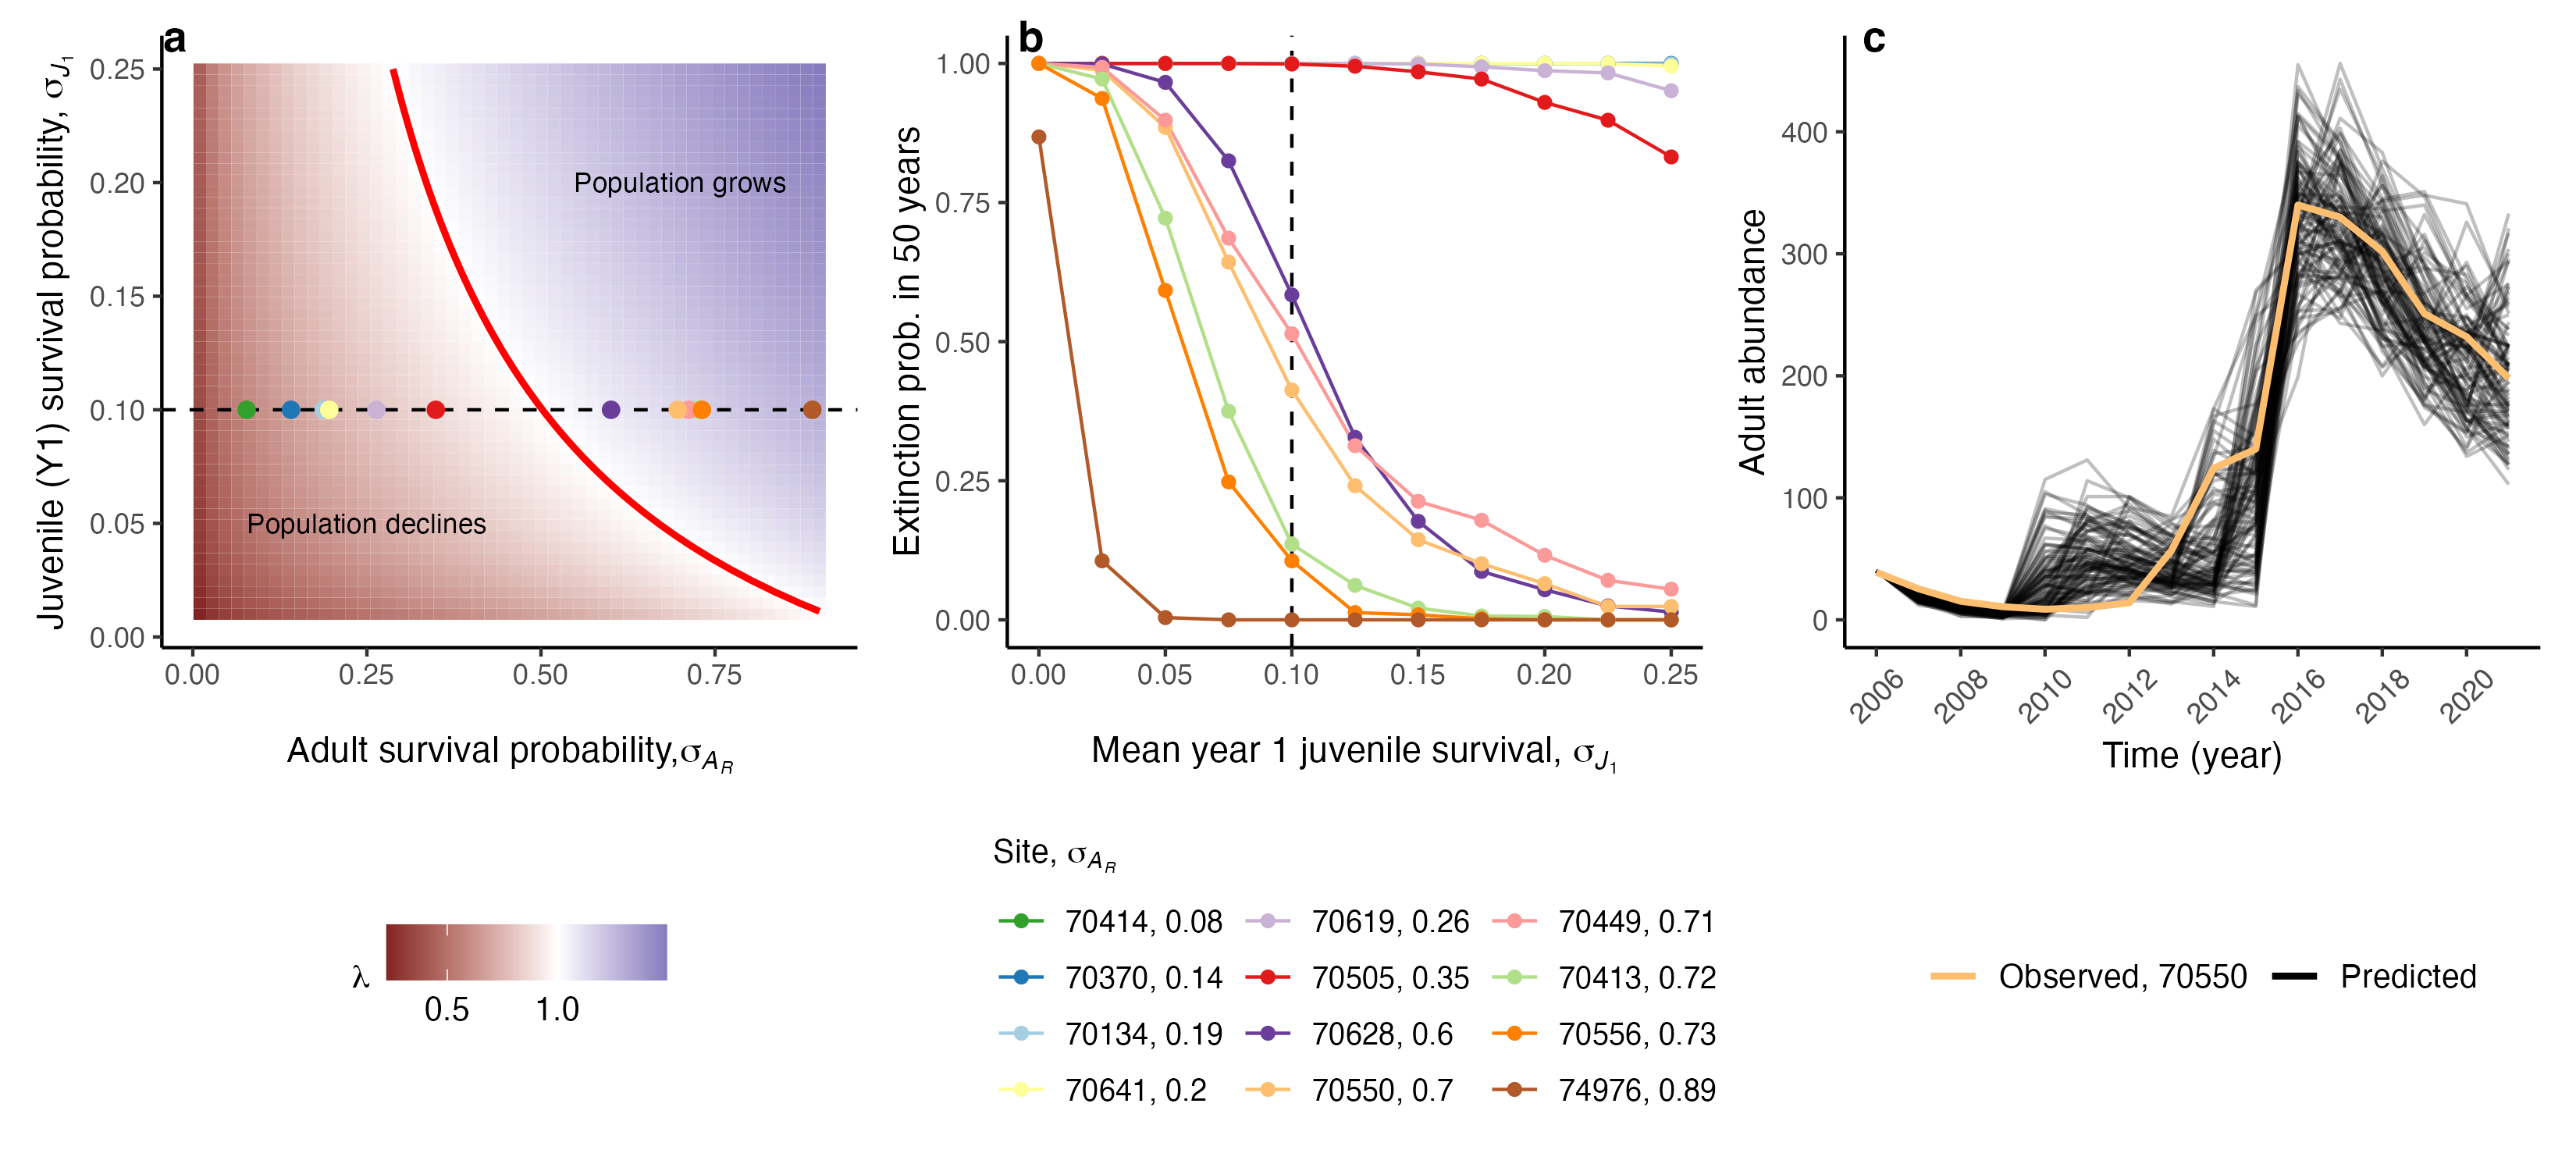
\includegraphics[width=0.95\textwidth,height=\textheight]{figures/pop_viability_figures_for_manuscript.png}

}

\caption{\label{fig-viability}\textbf{Estimated growth rates and
extinction probabilities of reintroduced populations}. \textbf{a}
Predicted long-run growth rate \(\lambda\) for different values of
yearly adult survival probability \(\sigma_{A_R}\) and year-1 juvenile
survival probability \(\sigma_{J_1}\), given the parameterized,
deterministic model. Colored points show the predicted \(\lambda\)
values for the twelve translocated populations when year-1 juvenile
survival probability is \(\sigma_{J_1} = 0.10\) (indicated by the dashed
line). The red line shows where \(\lambda = 1\). Note that the point for
70413 is mostly hidden behind other points. \textbf{b} Predicted 50-year
extinction probabilities of the 12 reintroduced populations, given
demographic stochasticity, environmental variability in
\(\sigma_{J_1}\), and different mean values of \(\sigma_{J_1}\). There
are 6 lines at extinction probability = 1, 5 of which (70414--70619) are
partially or completely hidden beneath the line for 70505. \textbf{c}
100 simulated trajectories (black lines) from the population viability
model that most closely matched the observed abundance trajectory of
adult amphibians at site 70550 (light orange).}

\end{figure}%




\end{document}
